%----------------------------------------
% SECTION: Toric Code and its features
%----------------------------------------
\section{Toric Code and its features}
\label{sec:toric_code_and_its_features}

The Toric code is two-dimensional model of spin-\onehalf degrees of freedom (d.o.f), which can be regarded as an example of a pure $\mathbb{Z}_2$ lattice gauge theory.
In particular, we focus on a $L \times L$ square lattice with periodic boundary conditions.
The \dof are defined on the links the lattice, where the local Hilbert space is $\C^2$.
The main operators we are going to use are the Pauli matrices
\begin{equation}
    X = \begin{pmatrix}
        0 & 1 \\ 1 & 0
    \end{pmatrix}
    \qand
    Z = \begin{pmatrix}
        1 & 0 \\ 0 & -1
    \end{pmatrix},
    \label{eq:matrices_X_Z}
\end{equation}
which we have written in the computational basis $\{\ket{0}, \ket{1}\}$, where the $Z$-matrix is diagonal.
It is important to remember that the matrices $X$ and $Z$ \emph{anticommutes}.
\begin{equation}
    [X, Z] = 0.
\end{equation}

The main \emph{local} operators that enters the Hamiltonian are defined on the \emph{stars} and \emph{plaquettes} of the lattice.
The term \emph{star} refers to the links attached to a common vertex $v$, while by \emph{plaquette} $p$ we mean the links around a face of the lattice.
A \emph{star operator} and a \emph{plaquette operator} are respectively defined as
\begin{equation}
    A_v = \prod_{\link \in s} Z_\link, \qquad
    B_p = \prod_{\link \in p} X_\link.
    \label{eq:star_plaq_op_def}
\end{equation}
where $v$ is a vertex and $p$ a plaquette (see Fig.~\ref{fig:toric_code_operators}).
One can easily see that
\begin{equation}
    \comm{A_v}{A_{v^{\prime}}} = 0 \qand
    \comm{B_p}{B_{p^{\prime}}} = 0
    \label{eq:star_plaq_op_comm_1}
\end{equation}
for all vertices $v$ and $v^{\prime} $, and all plaquettes $p$ and $p^{\prime} $.
But it is also true that
\begin{equation}
    \comm{A_v}{B_p} = 0
    \label{eq:star_plaq_op_comm_2}
\end{equation}
for all $v$ and $p$.
This is because a star and a plaquette share zero or two links, so the signs factors from the anticommutation of $X$ and $Z$ cancel out.
The eigenvalues of the Pauli matrices are just $\pm 1$, so the same holds true for $A_s$ and $B_p$.
Moreover, like the Pauli matrices, also $A_s^2 = \identity$ and $B_p^2 = \identity$.


Now, given the operators in \eqref{eq:star_plaq_op_def}, we can write down the Hamiltonian of the Toric Code:
\begin{equation}
    H = - \sum_{v} A_v - \sum_{p} B_p
    \label{eq:toric_code_hamiltonian}
\end{equation}
which is \emph{exactly solvable}, due to \eqref{eq:star_plaq_op_comm_1} and \eqref{eq:star_plaq_op_comm_2}.
\begin{figure}[t]
    \centering
    \begin{tikzpicture}[
        scale=1.2,
        site/.style = {circle, inner sep=0 pt, minimum size=3pt, draw=black, fill=white},
        plaq/.style={blue, ultra thick},
        gauss/.style={red, ultra thick}
        ]
    % Lattice
    \draw[thin] (-0.5,-0.5) grid (4.5,2.5);

    % Plaquette operator
    \draw[plaq] (3,1) -- (4,1) node [pos=0.5, below] {$X$};
    \draw[plaq] (4,1) -- (4,2) node [pos=0.5, right] {$X$};
    \draw[plaq] (4,2) -- (3,2) node [pos=0.5, above] {$X$};
    \draw[plaq] (3,2) -- (3,1) node [pos=0.5, left]  {$X$};
    \draw[blue, ultra thick, pattern=north east lines, pattern color=blue] (3,1) rectangle (4,2);
    \draw (3.5,1.5) node [fill=white, rounded corners] {$B_p$};

    % Gauss operator
    \draw[gauss] (1, 1) -- (2, 1) node [pos=0.5, below right] {$Z$};
    \draw[gauss] (1, 1) -- (1, 2) node [pos=0.5, above left] {$Z$};
    \draw[gauss] (1, 1) -- (0, 1) node [pos=0.5, below left] {$Z$};
    \draw[gauss] (1, 1) -- (1, 0) node [pos=0.5, below right] {$Z$};

    \foreach \y in {0,1,2} \foreach \x in {0,1,...,4} \draw (\x,\y) node [site] {};

    \draw (1,1) node [above right, outer sep=5pt, inner sep=3pt, draw=red, rounded corners=3pt] {$A_s$};
\end{tikzpicture}

    \caption{Graphical representation of the Toric Code operators $A_s$ and $B_p$}
    \label{fig:toric_code_operators}
\end{figure}



%
% SUBSECTION: Topological ground states
%
\subsection{Topological Ground states}
\label{sub:topological_ground_states}

Given the commutation relations of the $A_v$ and $B_p$ operators in \eqref{eq:star_plaq_op_comm_1} and \eqref{eq:star_plaq_op_comm_2}, one can find the ground state $\ket{\Omega}$ by simply imposing the constraints
\begin{equation}
    A_v \ket{\Omega} = \ket{\Omega} \qand
    B_p \ket{\Omega} = \ket{\Omega}, \qquad \forall v,\, p.
    \label{eq:ground_state_constraints}
\end{equation}
Even more, we can define the space of ground states
\begin{equation}
    \mathcal{L} = \qty{ \ket{\Omega} : A_s \ket{\Omega} = \ket{\Omega}, \quad B_p \ket{\Omega} = \ket{\Omega} \quad \forall s, p },
\end{equation}
which contents \emph{depends on the topology of the lattice}.
For example, we will see that with periodic boundary conditions, then there are $4$ degenerate ground states.
These degenerate ground states can only be distinguished with non-local operators.
This mechanics will be illustrated in the following.


Consider a torus geometry for the lattice of size $L \times L$, i.e.~periodic boundary conditions in both directions.
From \eqref{eq:ground_state_constraints}, we have $2L^2$ constraints but these are not all independent.
Indeed, if we multiply all the constraints on a torus we obtain
\begin{equation}
    \prod_{v} A_v = \identity \qand
    \prod_{p} B_p = \identity,
\end{equation}
which actually means that there are $2L^2 - 2$ independent conditions.
The total Hilbert space has dimension $2^{2L^2}$, therefore the space $\mathcal{L}$ has dimension $2^{2L^2 - 2L^2 + 2} = 4$, which means that the Toric Code has $4$ degenerate ground states.
On these states, the operators $A_v$ and $B_p$ have all the same eigenvalues and any other local operator that commutes with the Hamiltonian is given by a product of $A_v$ and $B_p$.
This in turn means that the degenerate ground states $\ket{\Omega} \in \mathcal{L}$ \emph{cannot be distinguished by local operators}.
The presence of this kind of degenerate ground states is a common feature of topological phases in two dimensions\citneeded.

In order to distinguish these ground states, it is necessary to find \emph{non-local operators} that commute with the Hamiltonian in \eqref{eq:toric_code_hamiltonian}.
Non-local in this instance means not expressible as a product or sum of vertex and plaquette operators.
But first let look more closely to the nature of \emph{local operators}.

Consider any region $\mathcal{R}$ on the lattice $\lattice$.
On this region $\mathcal{R}$ we can define a local operator $W$ as a product of $B_p$ operators:
\begin{equation}
    W = \prod_{p \in \mathcal{R}} B_p.
\end{equation}
Due to $X^2 = \identity$, this is equivalent to
\begin{equation}
    W = \prod_{\link \in \partial \mathcal{R}} X_{\link}.
\end{equation}
In other words, $W$ is equivalent to the product of $X$s along the closed curve (or multiple closed curves if $\mathcal{R}$ is disconnected) given by the boundary $\partial \mathcal{R}$ of $\mathcal{R}$.
In fact, the $B_p$ themselves are defined as product of $X$s along a closed curve, the plaquette.
In a sense, they are all \emph{string operators}.
The same argument can be repeated for $A_v$ on the dual lattice $\tilde{\lattice}$.
Indeed, a star on the direct lattice becomes a plaquette on the dual lattice.
So a product of $A_v$ is equivalent to a string of $Z$ operators along closed curves on the dual lattice.

All these curve have a common property, they are \emph{contractible}.
They can be reduced to a single point.
We can then conclude that what we have considered as local operators are indeed string operators on contractible curves.
But if we are on a lattice with non-trivial topology, like a torus, then we can also have \emph{non-contractible} curves.





% These ground states can only be distinguished by non-local operators that have to commute with Hamiltonian in \eqref{eq:toric_code_hamiltonian}, hence with all $A_v$ and $B_p$ but cannot be expressed in terms of $A_v$ and $B_p$.
The only operators that satisfy this requirements are defined on closed paths, on the direct or dual lattice, that cannot be reduced to a single plaquette loop (on the dual lattice the plaquettes are the stars of the direct lattice).
In other words, they are defined along \emph{non-contractible loops}.
The reason being that any product of $\sigma^x$ or $\sigma^z$ along a closed curve $\mathcal{C}$ that commutes with the Hamiltonian can be expressed as product of $A_v$ or $B_p$ of the stars or plaquettes enclosed by $\mathcal{C}$.
Consider now, two non-contractible curves $\mathcal{C}_{1}$ and $\mathcal{C}_{2}$ along the $\hat{1}$ and $\hat{2}$ direction respectively.
On these paths we can define the \emph{string operators}
\begin{equation}
    \overline{X}_1 = \prod_{j \in \mathcal{C}_1}  \sigma^x_j, \qquad
    \overline{X}_2 = \prod_{j \in \mathcal{C}_2}  \sigma^x_j,
    \label{eq:nonlocal_X_operators}
\end{equation}
it can be proved that they commute with all the local operators but cannot be expressed as a product of them.
The same can be repeated on the dual lattice, by considering dual non-contractible paths $\tilde{\mathcal{C}}_1$ and $\tilde{\mathcal{C}}_2$ and defining
\begin{equation}
    \overline{Z}_1 = \prod_{j \in \mathcal{\tilde{C}}_1}, \qquad
    \overline{Z}_2 = \prod_{j \in \mathcal{\tilde{C}}_2}
    \label{eq:nonlocal_Z_operators}
\end{equation}
Likewise, the operators in \eqref{eq:nonlocal_Z_operators} commutes with all the vertex and plaquettes operators but they do not commute with the X-operators in \eqref{eq:nonlocal_X_operators}.

In fact, \eqref{eq:nonlocal_X_operators} and \eqref{eq:nonlocal_Z_operators} have the same (anti)commutation relations of two qubits:
\begin{equation}
    \qty{ \overline{X}_1, \overline{Z}_2 } = 0, \qquad
    \qty{ \overline{X}_2, \overline{Z}_1 } = 0,
\end{equation}
Therefore, the Toric Code (on a torus) has a protected subspace $\mathcal{L}$ (the space of the ground states) that behaves like the Hilbert space of two qubits and the operators \eqref{eq:nonlocal_X_operators} and \eqref{eq:nonlocal_Z_operators} acts like unitary gates on this space.

\begin{figure}[t]
    \centering
    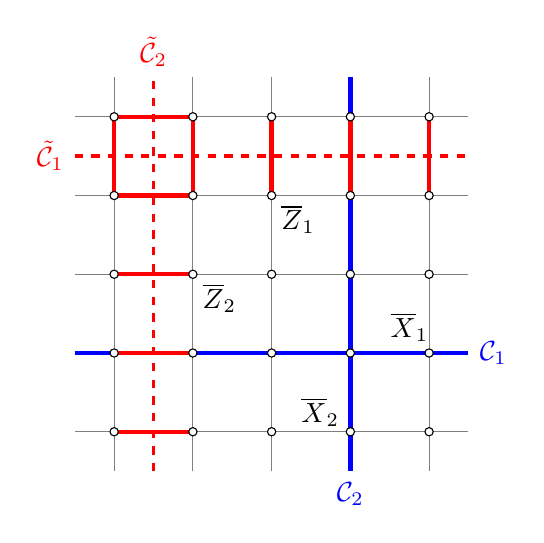
\begin{tikzpicture}[
        site/.style = {circle, inner sep=0 pt, minimum size=3pt, draw=black, fill=white},
    ]
    % lattice grid
    \draw[Gray,thin] (-0.5,-0.5) grid (4.5,4.5);

    % Wilson loops
    \draw[Blue, ultra thick]
        (-0.5, 1) -- (4.5, 1)
        node [pos=1, right] {$\mathcal{C}_1$}
        node [pos=0.85, above, black] {$\overline{X}_1$}
        ;
    \draw[Blue, ultra thick]
        (3, -0.5) -- (3, 4.5)
        node [pos=0, below] {$\mathcal{C}_2$}
        node [pos=0.15, left, black] {$\overline{X}_2$}
        ;

    % 't Hooft strings
    \draw[Red, very thick, dashed]
        (-0.5,3.5) -- (4.5,3.5)
        node[pos=0, left] {$\tilde{\mathcal{C}}_1$}
        ;
    \foreach \x in {0,...,4} { \draw[Red, ultra thick] (\x, 3) -- +(0, 1); }
    \draw (2,3) node [below right] {$\overline{Z}_1$};
    \draw[Red, very thick, dashed]
        (0.5,-0.5) -- (0.5,4.5)
        node[pos=1, above] {$\tilde{\mathcal{C}}_2$}
        ;
    \foreach \y in {0,...,4} { \draw[Red, ultra thick] (0, \y) -- +(1, 0); }
    \draw (1,2) node [below right] {$\overline{Z}_2$};
    \foreach \y in {0,...,4} \foreach \x in {0,...,4} \draw (\x,\y) node [site] {};
\end{tikzpicture}

    \caption{Non-contractible paths}
\end{figure}

\todo{revisionare}



\subsection{Particle excitations}%
\label{sub:particle_excitations}

Until now we have only discussed the ground states of the Toric Code, without touching the rest of the low energy sectors.
In other words, how do we describe the excitations of this model?
As we said, \eqref{eq:ground_state_constraints} are the set of constraints that defines the ground states.
Therefore, everytime a given state $\ket{\Psi}$ violates these equations, we will say that it contains \emph{particles}, which can be of different types.
If $A_v \ket{\Psi} = - \ket{\Psi}$, then we will say that the vertex $v$ contains a $z$-type particle.
Likewise, if $B_p \ket{\Psi} = - \ket{\Psi}$, then the plaquette $p$ contains a $x$-type particle.

Now the question: starting from a ground state $\ket{\Omega}$, how can we introduce some particles?
The answer is \emph{string operators}.
We are not considering closed strings, like we did in Sec.~\ref{sub:topological_ground_states}, but any open string.
The shortest open string that we can consider is a single link.
So a $Z$-string on a single link is just $Z_j$, where $j$ is a label of a generic link.
Consider now the state
\begin{equation}
    \ket*{\Psi^Z} = Z_j \ket{\Omega},
\end{equation}
This state hosts particles at the ``boundaries'' of the $j$-th link, i.e.~the vertices touching $j$ which we call $v_0$ and $v_1$.
This can be proved by simply showing that $[ A_v, Z_j ] = 0$ for $v \neq v_0$ and $v \neq v_1$ and $\{ A_{v_0}, Z_j \} = \{ A_{v_1}, Z_j \} = 0$.
Which immediately implies that
\begin{equation}
    A_{v_0} \ket*{\Psi^Z} = A_{v_1} \ket*{\Psi^Z} = - \ket*{\Psi^Z}
\end{equation}

